%Beschreibung der Implementierung der SPH-Flüssigkeitssimulation

\section{Partikel-basierte Simulation}
Es gibt zwei grundlegende Ansätze für die Simulation von Flüssigkeiten: entweder auf Gittern oder auf Partikeln basierend. Die Repräsentation von Simulationen in einem Gitter ist genauer, jedoch ebenso rechenintensiver \cite{fluid.tutorial_paper}. Da dieses Projekt auf Mikrocontrollern umgesetzt und die Flüssigkeit auf einem Bildschirm mit niedriger Auflösung angezeigt werden soll fiel die Wahl auf die Partikel-basierte Simulation.

\subsection{Grundlagen}

Die Simulation von Flüssigkeiten beruht auf den Navier Stokes Gleichungen \cite{fluid.tutorial_paper}\footnote{$\overrightarrow{u}$ ist die Geschwindigkeit der Flüssigkeit, $\rho$ die Dichte. Der Druck innerhalb der Flüssigkeit wird durch $p$ dargestellt und $v$ entspricht der kinematische Viskosität}: 

\begin{align}
	\frac{\partial \overrightarrow{u}}{\partial t} + \overrightarrow{u} + \frac{1}{\rho} \nabla p &= \overrightarrow{F} + v \nabla \cdot \nabla \overrightarrow{u} \\
	\nabla \cdot \overrightarrow{u} &= 0
\end{align}

\cite{fluid.website} und \cite{fluid.website2} führt aus, wie mit Hilfe der Kernel \texttt{poly6}, \texttt{spiky} und \texttt{viscosity} die folgenden Formeln für die Dichte, den Druck und die Viskosität erstellt werden können:

\begin{align}
	\rho_i &= \sum^{j} m_j W(|r_i - r_j|, h) \\
	F_i^{pressure} &= - \sum^{j} m_i m_j (\frac{p_i}{\rho_j^2} + \frac{p_j}{\rho_j^2}) \nabla W(|r_i - r_j|, h) \\
	F_i^{viscosity} &= \eta \sum^{j} m_j \frac{|u_j - u_i|}{\rho_j} \nabla^2 W(|r_i - r_j|, h)
\end{align}

Für die einzelnen Kernel gilt:
\begin{align}
	W_{poly6}(r, h) &= \frac{315}{56 \pi h^9} 	\begin{cases}
													(h^2 - r^2)^3,   & 0 \leq r \leq h\\
													0, & \text{andernfalls}\\
												\end{cases} \\
	W_{spiky}(r, h) &= \frac{15}{\pi h^6}		\begin{cases}
													(h - r),   & 0 \leq r \leq h\\
													0, & \text{andernfalls}\\
												\end{cases} \\
	W_{viscosity}(r, h) &= \frac{15}{2 \pi h^3}		\begin{cases}
													-\frac{r^3}{2h^3} + \frac{r^2}{h^2} + \frac{h}{2r} - 1,   & 0 \leq r \leq h\\
													0, & \text{andernfalls}\\
												\end{cases}
\end{align}

Ein Problem in der Simulation ist, dass alle Partikel auf alle anderen einwirken. Dies stellt eine $O(n^2)$ Beziehung da, die sich sehr negativ auf den Rechenaufwand auswirkt. Ein Weg die Berechnung zu Beschleunigen beruht auf dem Fakt, dass der Einfluss von entfernteren Partikeln auf das gerade betrachtete stetig abnimmt. Wenn man nun die aktuelle Position der Partikel auf einem Schachbrett aufträgt, so reicht es nur die Partikel, die sich in den umliegenden Feldern befinden, in die Berechnung der Kräfte die auf einen gegebenen Partikel wirken, zu betrachten.

\subsection{Umsetzung}

Die Simulation der Partikel wurde in \texttt{C} für den 2D-Raum umgesetzt. In einem 2D-Array sind in jedem Eintrag doppelt verkettete Listen aus den Partikeln verlinkt, die sich aktuell innerhalb dem Feld befinden (siehe \ref{code.sph.structs}). Zur Berechnung der nächsten Position eines jeden Partikels werden Dichte, Druck und Viskosität des Partikels unter Berücksichtigung der Umliegenden berechnet. Addiert man nun die soeben berechneten Kräfte mit der extern Einwirkenden (Erdanziehungskraft) und integriert dies über die verstrichene Zeit erhält man den Beschleunigungsvektor des Teilchens. Die Multiplikation der Beschleunigung mit der verstrichenen Zeit ergibt nun die Positionsveränderung des Partikels.

\begin{lstlisting}[language={c}, caption={Datenstrukturen der SPH}, label={code.sph.structs}]
typedef struct
{
	double position[2];
	double velocity[2];
	double mass;
	double density;
	double pressure;
	double force[2];
} particle_t;


typedef struct particle_list_element_s
{
	particle_t particle;
	struct particle_list_element_s* prev;
	struct particle_list_element_s* next;
} particle_list_element_t;


typedef struct
{
	particle_list_element_t* particle_list;
	uint32_t particle_count;
} particle_grid_element_t;

typedef particle_grid_element_t panel_t[PARTICLE_GRID_X][PARTICLE_GRID_Y];
\end{lstlisting}

\begin{wrapfigure}{r}{0.5\textwidth}
	\centering
	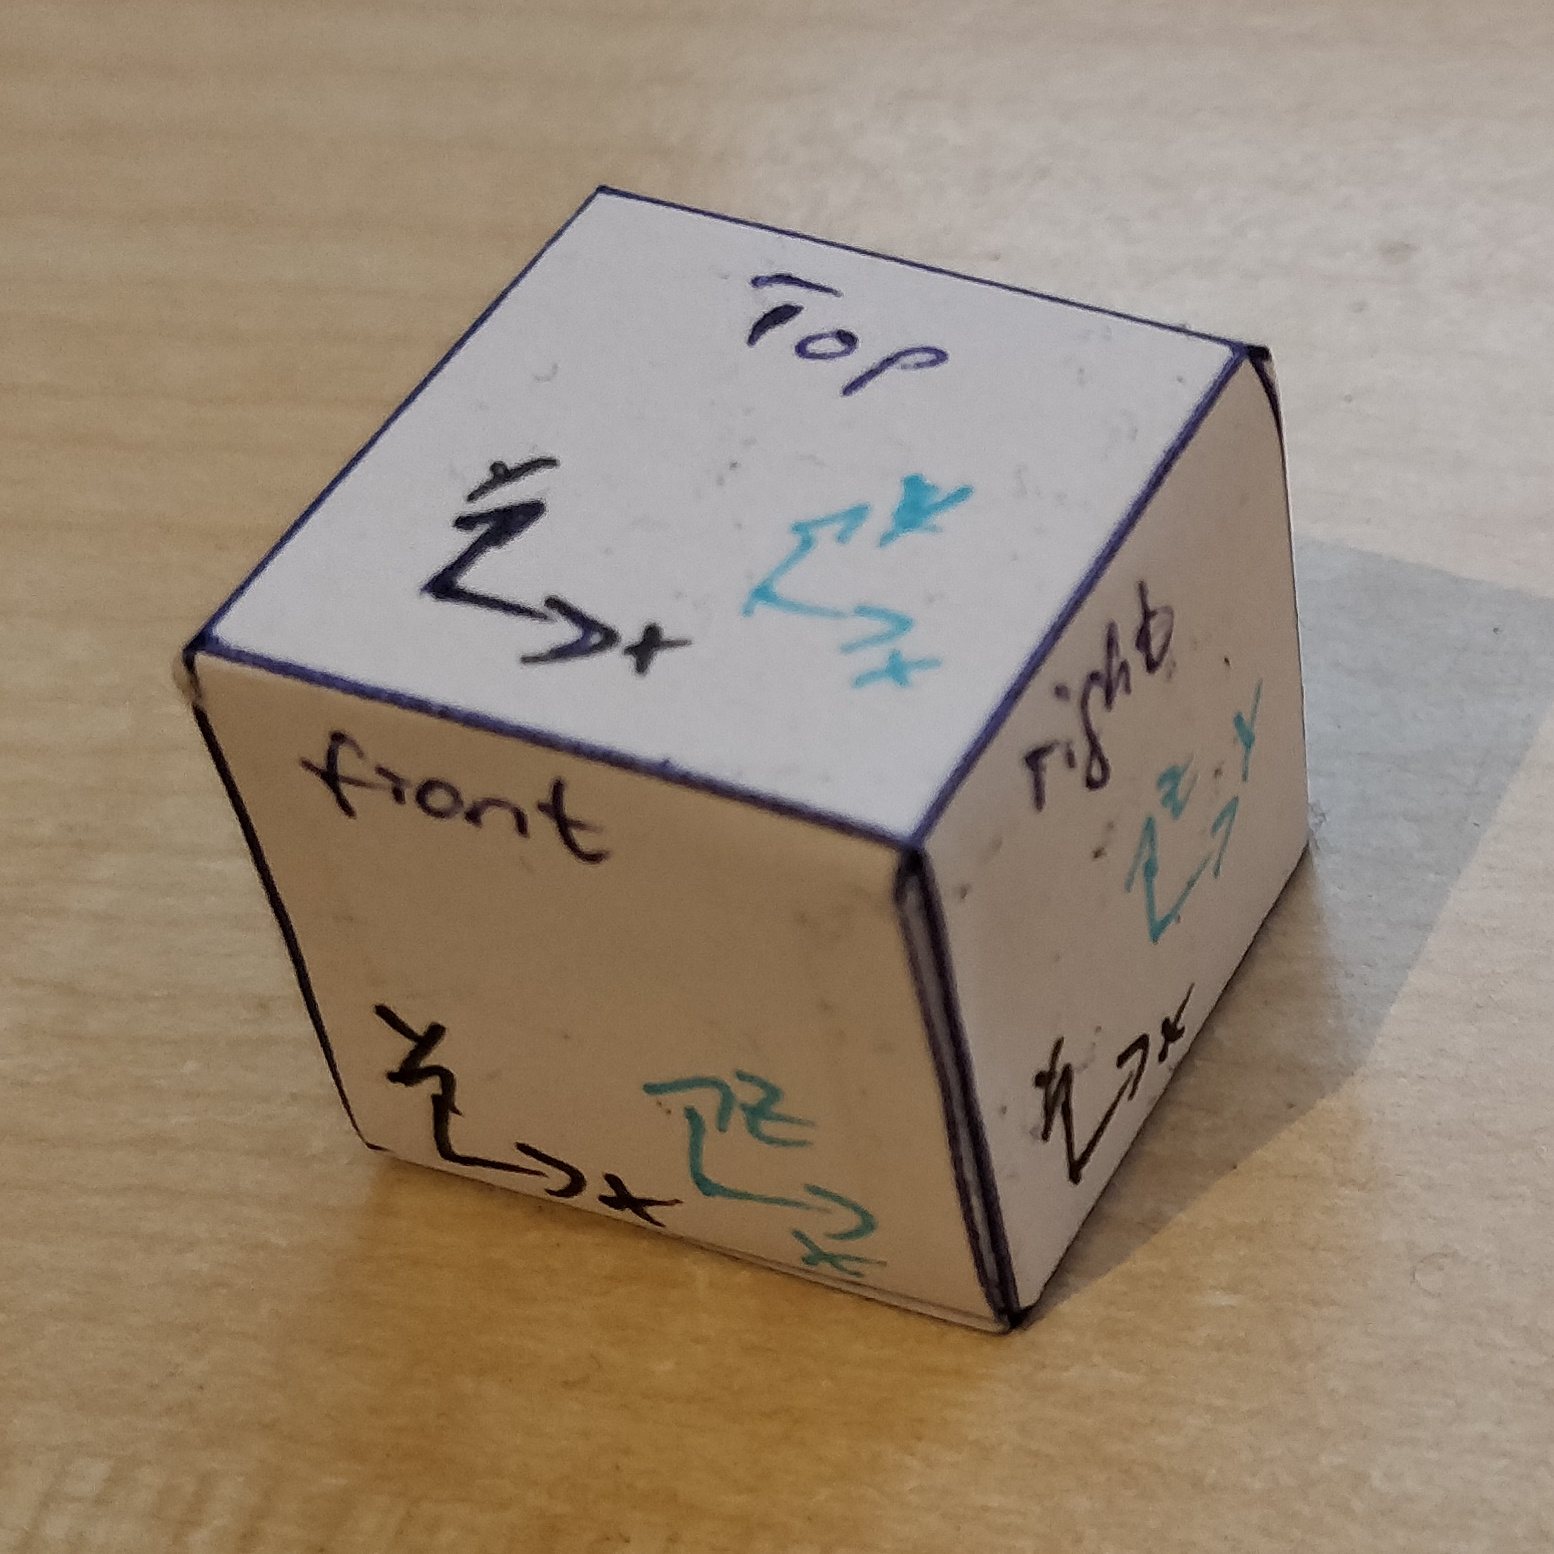
\includegraphics[width=.45\linewidth]{IMG_20190409_212603.jpg}
	\caption{Würfelmodell mit Koordinatensystem der LED-Panels und der 2D-Arrays}
	\label{fig:sph:cube_model}
\end{wrapfigure}

Um den Würfel darzustellen werden nun sechs der 2D-Arrays genutzt. Wenn die neue Position eines Partikels nun die Außengrenzen des Arrays überschreiten würde, so wird es auf die andere Würfelseite übertragen. Die Implementierung der Simulation wurde während der Entwicklung auf einem Linux-PC getestet. Hierzu wurde sie in ein Programm eingebettet, die Position der einzelnen Partikel ausließt und über X11 auf dem Bildschirm darstellt. Da die Simulation nur mit elementaren Rechenoperationen arbeitet konnte sie im Anschluss problemlos in das ARM-Programm eingefügt werden. Dieses stellt nun die Anzahl der Partikel in einem Feld der 2D-Arrays als Farbschattierung auf dem LED-Display dar.

\subsection{Rechenbeschleunigung durch RaspberryPi 1B}
\label{chap:impl:sph:rp}
\FloatBarrier

\begin{lstlisting}[caption={Memorymap des Raspberry Pi 1B}, label={code.sph.rp.memmap}]
MEMORY
{
	ram : ORIGIN = 0x8000, LENGTH = 0x1000
}

SECTIONS
{
	.text : { *(.text*) } > ram
	.bss  : { *(.bss* ) } > ram
}
\end{lstlisting}

\begin{lstlisting}[language={[ARM]{Assembler}}, caption={ARM ASM startup code}, label={code.sph.rp.startup}]
.globl _start
_start:
	ldr sp, stack_start
	ldr r0, thumb_start_add
	bx r0

stack_start: .word 0x8000
thumb_start_add: .word thumb_start
	.word 0
	.word 0

.thumb
.thumb_func
thumb_start:
	bl main
hang: b hang

\end{lstlisting}

\begin{figure}
	\begin{bytefield}[bitwidth=1.1em]{32}
		\bitheader{0-31} \\
		\wordbox{1}{sync-marker \tiny{\texttt{0xF3CFC3CF}}} \\
		\bitbox{8}{panel\_no} & \bitbox{8}{x\_position} & \bitbox{8}{y\_position} & \bitbox{8}{color} \\
		\bitbox[lrb]{24}{color}
	\end{bytefield}
	\caption{Raspberry Pi Pixeldaten}
	\label{fig:sph:rp:pixels}
\end{figure}

\begin{figure}
	\begin{bytefield}[bitwidth=1.1em]{32}
		\bitheader{0-31} \\
		\wordbox{1}{sync-marker \tiny{\texttt{0xF3CFC3CF}}} \\
		\wordbox{1}{force\_x \tiny{(double)}} \\
		\wordbox{1}{force\_y \tiny{(double)}} \\
		\wordbox{1}{force\_z \tiny{(double)}}
	\end{bytefield}
	\caption{MCB2388 Accelerometer Daten}
	\label{fig:sph:rp:acc_data}
\end{figure}

Mit der Zusammenführung aller Teilkomponenten (siehe auch die Kapitel \nameref{chap:impl:accel} und \nameref{chap:impl:ledcube}) wurde klar, dass die maximale Taktung des genutzten \texttt{LPC2388} zwar gerade so für eine flüssige Darstellung auf dem Würfel ausreicht, jedoch die Berechnungen der Simulation zu merklichen Stottern ($\geq 250$ms) führt. Auch das Triggern der Bildwiederholung via Timer-Interrupt führte zu keinem zufriedenstellendem Ergebnis: eine flüssige Darstellung war nur möglich, wenn der Intervall des Interrupts so weit hochgestellt wurde, dass er dauerhaft anliegt. Daraufhin entschieden wir uns die Simulation selber auf einen \texttt{Raspberry Pi 1B} auszulagern, da dieser mit einer Frequenz von $700$MHz getaktet ist, etwa $10$ mal höher als der \texttt{LPC2388}.

Der Pi ist, mit Hilfe von \cite{rp1.headless.github}, ohne Nutzung eines Betriebssystems programmiert worden. Auf ihm ist ein \texttt{BCM2835} als Prozessor mit integrierter GPU verbaut. Die GPU sicht auf der ersten Partition der FAT32 formatierten SD-Karte beim Startup nach den boot-dateien \texttt{bootcode.bin}, \texttt{config.txt} und \texttt{start.elf} und ließt anschließend die \texttt{kernel.img} und lädt diese in den Speicher. Nun wird der reset des ARMs freigegeben, dieser führt dann die \texttt{kernel.img} aus. \texttt{bootcode.bin}, \texttt{config.txt} und \texttt{start.elf} können ohne weiteres dem firmware-repository\footnote{Siehe \url{https://github.com/raspberrypi/firmware/tree/master/boot}, Zugriff am 10.04.2019} der raspberrypi-foundation entnommen werden. Die \texttt{config.txt} wird genutzt um die \texttt{UART} Schnittstelle zu initialisieren.

Der Programmcode wird mit dem \texttt{arm-none-eabi-gcc} kompilliert und gelinkt \footnote{Optionen: \texttt{-mfpu=vfp -march=armv6zk -mtune=arm1176jzf-s -nostdlib -nostartfiles -std=c99 -ffreestanding}}, die kernel.img wird aus der erstellten .elf mittels \texttt{arm-none-eabi-objcopy kernel.elf -O binary kernel.img} extrahiert. Hierbei ist es wichtig, beim Bauen der \texttt{.elf} eine Memorymap (Siehe \ref{code.sph.rp.memmap}) mit der Option \texttt{-T} mit einzubinden.

Die SPH Simulation wurde nun um eine Callback-option beim Wechsel eines Partikels zu einem anderen Feld erweitert. Diese löst eine Kommunikation mittels dem \texttt{UART} aus (\cite{rp1.headless.github}[uart04] und \cite{broadcom.bcm2835.user_manual}[S.177 ff]) die ein Update zu den betroffenen Pixeln zum \texttt{LPC2388} schickt (vgl. \ref{fig:sph:rp:pixels}). Letzterer überträgt in regelmäßigen Abständen die vom \texttt{ADXL345} (vgl. Kapitel \ref{chap:impl:accel}) ausgelesenen Werte an den Pi (vgl. \ref{fig:sph:rp:acc_data}). Das Empfangen dieser Bytes löst einen Interrupt aus, welcher diese parst und die Werte der externen Kräfte aktualisiert. Wenn der Pin \texttt{3.7} des \texttt{LPC2388} auf $3,3$V gezogen wird ist die lokale Simulation aktiviert, ansonsten die externe via \texttt{UART} Kommunikation.